\documentclass[11pt,letterpaper]{report}
\usepackage{amsfonts,amssymb,amsmath}
\usepackage{wasysym}
\usepackage{graphicx}
\usepackage{fancybox}
\usepackage[hidelinks]{hyperref}
\usepackage[usenames]{color}
\usepackage[utf8]{inputenc}

\begin{document}

	
	\begin{tabular}{l c r}
		
		
\includegraphics[scale=0.1]{ucvlogo.jpg} & \hspace{0.1cm}
		
		\begin{minipage}{6.6cm}
			\vspace{-1cm}
			\hspace{20cm}
			\centering\textbf{Universidad Central de Venezuela \\ Facultad de Ciencias \\ Introducci\'on a la Ciencia de Datos}
		\end{minipage} & \hspace{0.5 cm}
		
\includegraphics[scale=0.25]{images.jpg}
	\end{tabular}
	\\ \\ 
	
	
	\begin{center}
		\textbf{\large Proyecto de Ciencia de Datos\\
		 Agrupaci\'on de los jugadores de baseball de la MLB en la temporada regular 2016 de acuerdo a su rendimiento como bateadores}
	\end{center}  
	
	\begin{table}[h]
		\begin{tabular}{l l c r r}
			\textbf{} &\ \ \ \ \ \ \ \ \ \ \ \ \ \ \ \ \ \ \ \ \ \ \ \ \ \ \ \ \ \ \ \ \ \ \ \ \ \ \ \ \ \ \ \ \ \  \textbf{ }  & & \textbf{\large Autor:} & \textbf{\large Jorge Flores } \\ 
		\end{tabular}
	\end{table} 
	
	\begin{center}
		\textbf{\large Introducci\'on}
	\end{center}
	
	
	El baseball es un deporte en el cual toda acci\'on que se realiza queda \ \ \ registrada, esto ayuda a establecer una serie de estad\'isticas por jugador como el bateador, pitcher y sus respectivas posiciones. A su vez, por equipo quedan registradas las victorias, derrotas y otros tipos de logros, lo que hace al baseball muy interesante, ya que gracias a esta cualidad han surgido nuevas inquietudes para hacer este deporte m\'as efectivo que otros. \\ 
	
	Con un registro tan amplio de estad\'isticas, se trabajar\'a sobre la de los bateadores espec\'ificamente en el cual se aplicar\'a unas t\'ecnicas de miner\'ia de datos las cuales son conocidas como clustering, scraping web y clasificaci\'on donde el proceso de clustering es un m\'etodo de aprendizaje no supervisado el cual consiste en generar grupos que comparten caracter\'isticas similares para el conjunto de datos. El proceso de scraping web consiste en extraer todo tipo de informaci\'on de la web por medio de progaramas de software como R, Python entre otros, lo cual permite hacer un estudio con mayor rigurosidad. \\ 
	
	El motivo que inspir\'o a la realizaci\'on de este proyecto fue la aplicaci\'on de la Ciencia de Datos en el campo del deporte.
	De acuerdo a lo expuesto anteriormente, en este proyecto se plantea como objetivo agrupar y clasificar a los bateadores de Major League Baseball (MLB) de la temporada regular 2016 mediante la técnica de clustering. \\ \\ 
	
	\begin{center}
		\textbf{\large Planteamiento del problema}
	\end{center}
	
	 En la actualidad, los cient\'ificos de datos est\'an adquiriendo un roll muy importante en la vida cotidiana, ya que se requiere de sus especialidades para encontrar soluciones a problemas que antes no se hab\'ian tratado. Un ejemplo de ello es aplicar las t\'ecnicas Web scraping y clustering en el \'ambito deportivo, lo cual es importante ya que se puede encontrar nuevos clasificadores para los deportistas seg\'un su rendimiento, caracter\'isticas y potencial atl\'etico.\\
	 
	 Con base en lo anterior puede inferirse que el m\'etodo de clustering en el baseball ser\'a de gran ayuda para el an\'alisis t\'ecnico de los jugadores y realizar una mejor estrategia para el funcionamiento del equipo.\\ 
	  
	 
	 V\'asquez Fern\'andez, Miguel (2014) en su tesis de grado \textbf{"COMBINING CLUSTERING AND TIME SERIES FOR BASEBALL FORECASTING"} a partir de la t\'ecnica clustering, profundiz\'o en el tema de la Ciencia de Datos en el deporte. El principal aporte de esta investigaci\'on fue lograr predecir de manera favorable la complejidad de esta tarea. \\ 
	 
	 Otro material que fue tomado en cuenta como antecedente para este proyecto es la pel\'icula \textbf{"Moneyball"}, producida por Bennett Miller, Octubre 2011. Esta pel\'icula ofrece informaci\'on valiosa para el proyecto debido a que es basada en una historia de la vida real en la que se aplica an\'alisis estad\'istico en el baseball con el fin de formar un buen equipo con un presupuesto reducido.\\ 
	 
	 Dentro de esta perspectiva, el problema de la investigaci\'on puede ser formulado de la siguiente manera:\\
	  
	 ¿C\'omo se pueden agrupar a los jugadores de la MLB de la temporada regular 2016 seg\'un su rendimiento? \\ 
	 
	 De esta interrogante se desprenden las siguientes preguntas:\\
	  
	\noindent $\bullet$¿Qu\'e jugadores ser\'an tomados en cuenta para la realizaci\'on de proyecto? \\
	$\bullet$¿Cu\'ales son las caracter\'isticas a estudiar? \\ 
    $\bullet$¿C\'omo ser\'a la clasificaci\'on de los jugadores luego de los m\'etodos aplicados? \\ 
    
    Por otra parte, este proyecto busca generar respuestas c\'omo encontar una agrupaci\'on de los bateadores de acuerdo a su rendimiento tomando en cuenta los datos que quedan registrados como: en cu\'antos juegos particip\'o, cu\'antos turnos al bate tom\'o, cu\'antos hit conect\'o, cuantas carreras impuls\'o y otra serie de caracter\'isticas que ser\'an visualizadas mejor en la tabla de datos, esto se realizar\'a mediante el lenguaje de programaci\'on R en el cual se aplicar\'a la t\'ecnica web scraping para obtener los datos de la p\'agina oficial de la MLB que contiene toda la lista de los bateadores que participaron en la temporada regular 2016. Luego de dicha extracci\'on se procede al siguiente paso en el cual se preparar\'an los datos para realizar la investigaci\'on.\\
    
    Una vez culminado el procedimiento anterior, se aplicar\'a el algoritmo K-means y as\'i se encontrar\'an las diferentes agrupaciones de los bateadores lo cual permitir\'a clasificarlos seg\'un su capacidad de rendimiento.
    
   \begin{center}
   	\textbf{\large Procedimiento para la elecci\'on de los grupos}
   \end{center}
   
   Para realizar el trabajo de investigaci\'on se aplic\'o el algoritmo K-means, la elecci\'on del “k” se hace mediante el codo de Jambu, donde se puede visualizar en la siguiente gr\'afica que el “k” puede ser 4 \'o 5. En esta ocasi\'on se eligi\'o k=4 ya que cuando se dividi\'o a los jugadores en 5 grupos, ese grupo adicional era de 4 individuos los cuales no eran de gran relevancia  y solo disminuía el error en menos de 1\%.
   
   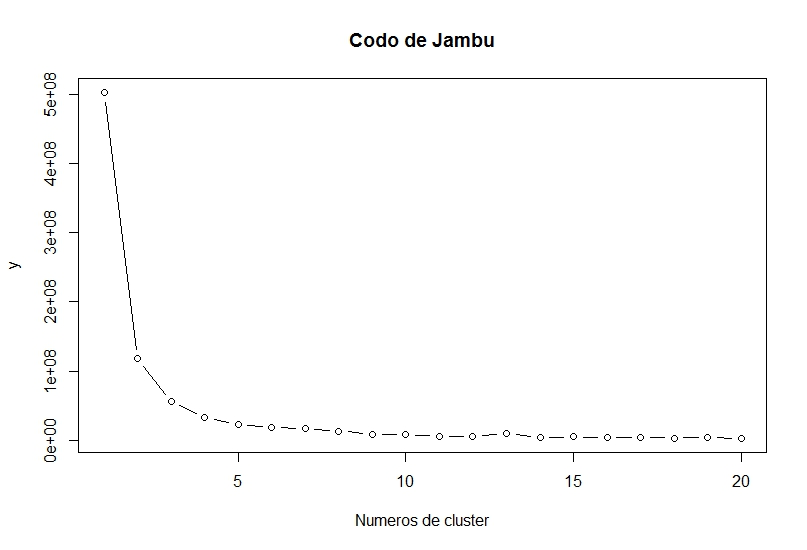
\includegraphics[scale=0.5]{Codo.jpeg}
   
   Esta gr\'afica permite observar los grupos con las observaciones de "AB" y "OPS"
   
   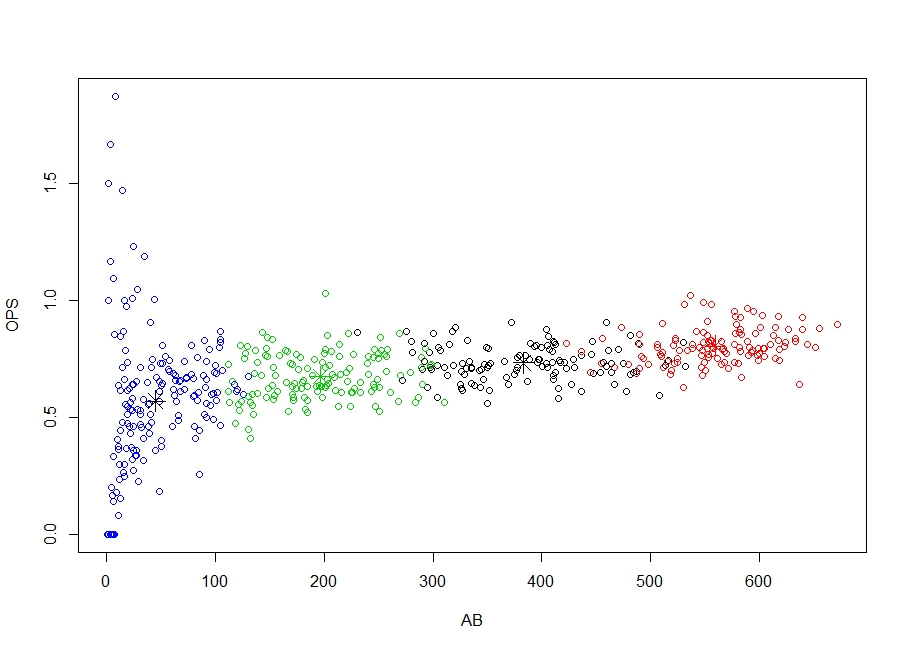
\includegraphics[scale=0.5]{Grupos.jpeg} \\
   
   
   \begin{center}
   	\textbf{\large Datos}
   \end{center}
   
   Para la realizaci\'on del proyecto se utiliz\'o la siguiente base de datos (\textcolor{cyan}{\underline{\href{http://mlb.mlb.com/stats/}{link}}}), en donde se encuentra reflejado el rendimiento de cada bateador de la MLB temporada regular 2016.\\ 
   
   A su vez, en este (\textcolor{cyan}{\underline{\href{http://m.mlb.com/player/408234/miguel-cabrera}{link}}}) se utilizan características específicas del jugador como: peso, estatura, entre otros.\\ 
   
   A continuación se presentan las imágenes de la tabla y del perfil del jugador donde se aprecian las estadísticas que serán utilizadas para la investigación. \\
   \\
   \\
  \begin{center}
  	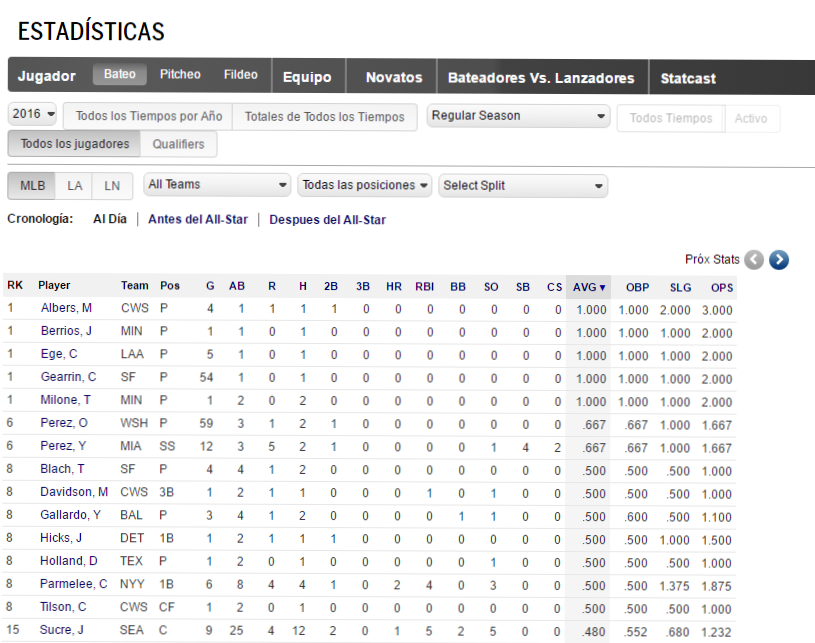
\includegraphics[scale=0.5]{vista.png} \\ \vspace{1.5cm}
  \end{center} 
  
  \begin{center}
     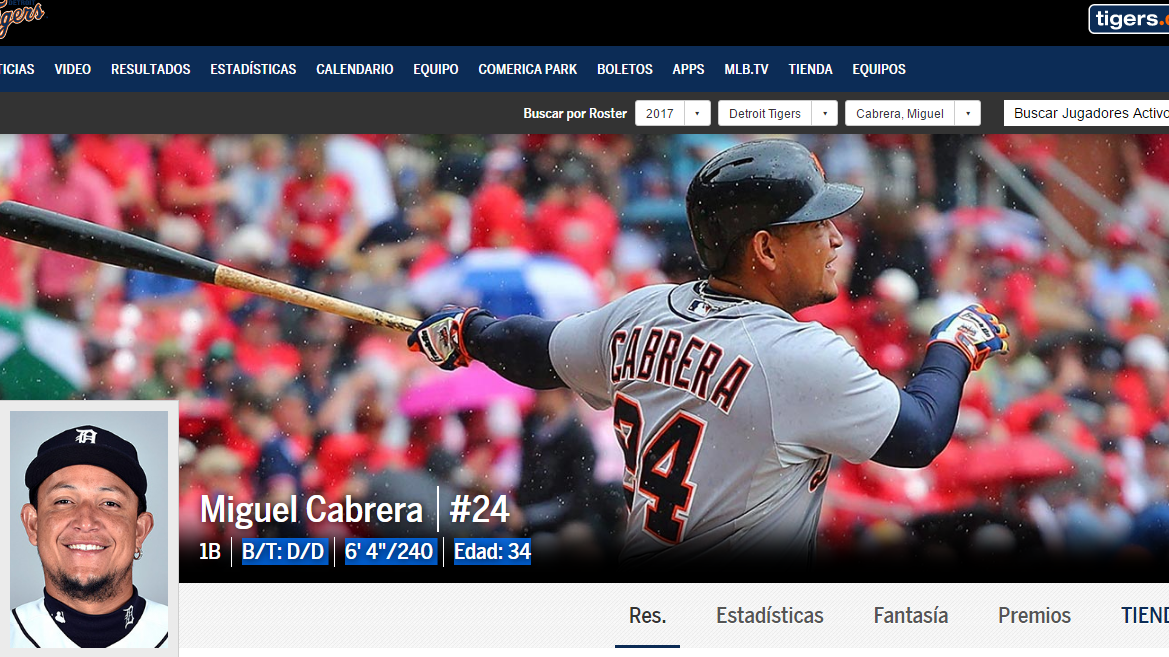
\includegraphics[scale=0.4]{2017.png}
  \end{center}
  \noindent \\ 
  
  
   El método que se aplicó para la extracción de los datos fue la técnica web scraping, la cual se llevó a cabo con la extensión de Google Chrome llamada Scraper totalmente gratuita. Hay otras formas de aplicar dicha técnica, una de ellas es en el lenguaje de programación Python utilizando los paquetes (Scrapy o Beatiful Soup), sin embargo, se eligió la extensión Scraper  ya que facilitó la obtención de los datos  de manera exitosa.\\ 
  
  Se puede apreciar un grafo en el cual se muestra como se obtuvieron los datos. \\ 
  
\begin{center}
	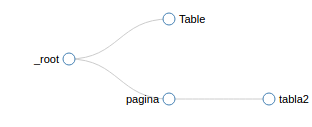
\includegraphics[scale=0.8]{grafo1.png} \\ \vspace{3cm}
	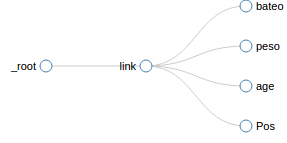
\includegraphics[scale=0.8]{grafo2.png}
\end{center} 
\noindent \\  



 Luego de la obtención de los datos se procede a ejecutar la limpieza, la cual fue realizada en el lenguaje de programación Python utilizando las bibliotecas (Pandas y Numpy). Para dicha limpieza se toman en cuenta las siguientes observaciones. Solo se trabajó sobre los jugadores que no ocupan la posición de pitcher, ya que hay una gran diferencia entre la cantidad de turnos al bate del pitcher con respecto a la cantidad  de turnos al bate de un jugador que ocupe otra posición. Por otra parte, se encontraron valores faltantes en la variable edad. Este problema se solucionó remplazando dichos valores por la moda, la cual era 26 años, a su vez, las variables peso y estatura  estaban representadas en el sistema inglés las cuales se transformaron en medidas del sistema métrico decimal. Para la lateralidad de los bateadores se le asignó: (diestro: $1$, zurdo: $-1$, ambidiestro: $0$), además se eliminaron jugadores duplicados.\\
 
 \textbf{Nota: El código de limpieza se encuentra en el siguiente (\textcolor{cyan}{\underline{\href{https://github.com/jorge13flores/Proyecto-Final/blob/master/Limpieza.ipynb}{link}}}).} 


\begin{center}
	\textbf{\large Análisis Exploratorio}
\end{center} 
    
   Luego de emplear la técnica de clustering se obtuvo un total de 4 grupos. 
   En las siguientes gráficas se puede observar el comportamiento que presenta cada grupo considerando las siguientes variables: (Juegos, Carreras, HR, AVG, OPS), identificando la recta como el promedio de todo el conjunto de datos en su respectiva variable.
   
    \begin{center}
    	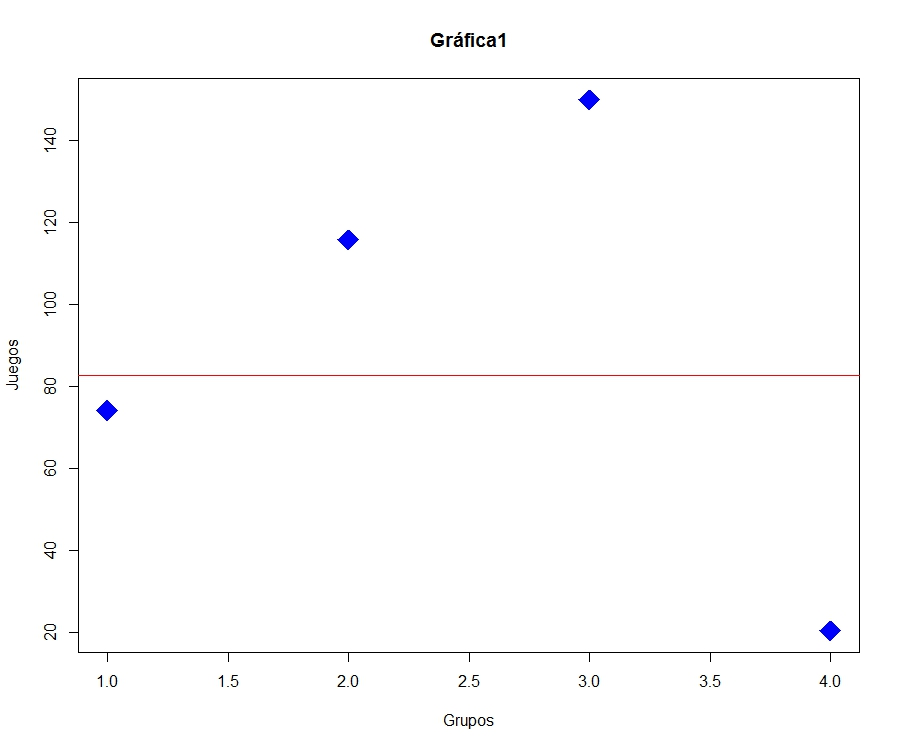
\includegraphics[scale=0.4]{Grafica1.jpeg} \\ \vspace{1.5cm}
    	
    	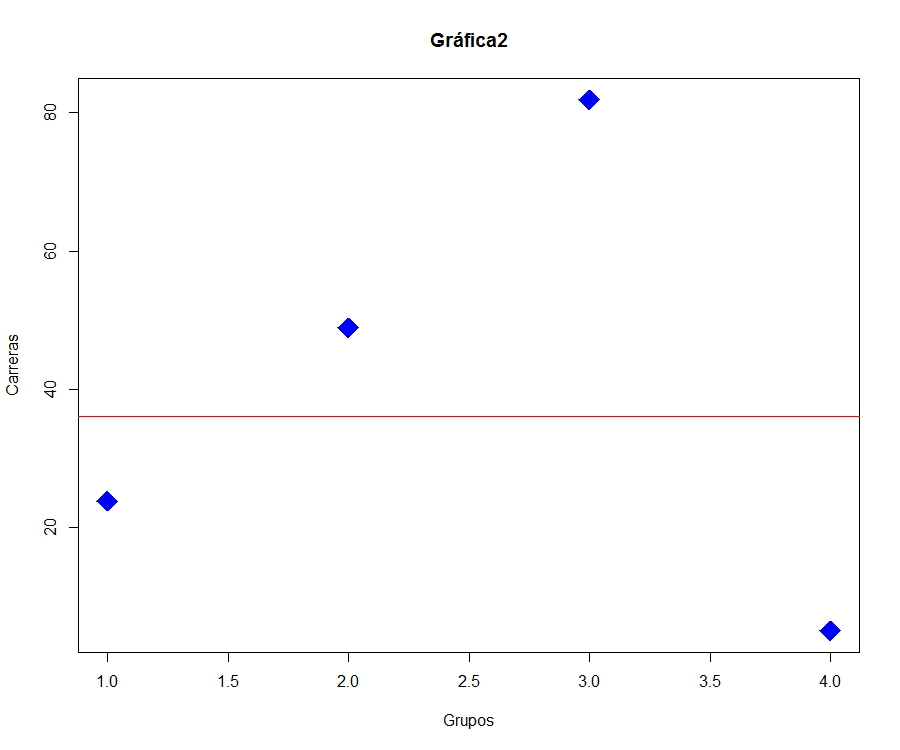
\includegraphics[scale=0.4]{Grafica2.jpeg} \vspace{1.5cm}
    	
    	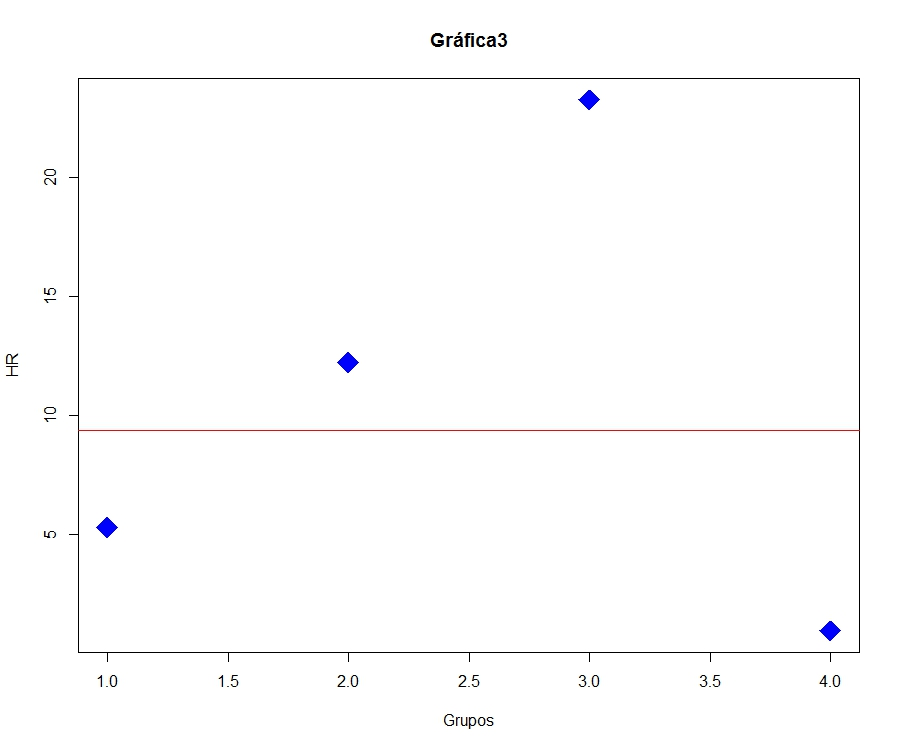
\includegraphics[scale=0.4]{Grafica3.jpeg} \vspace{1.5cm}
    	
    	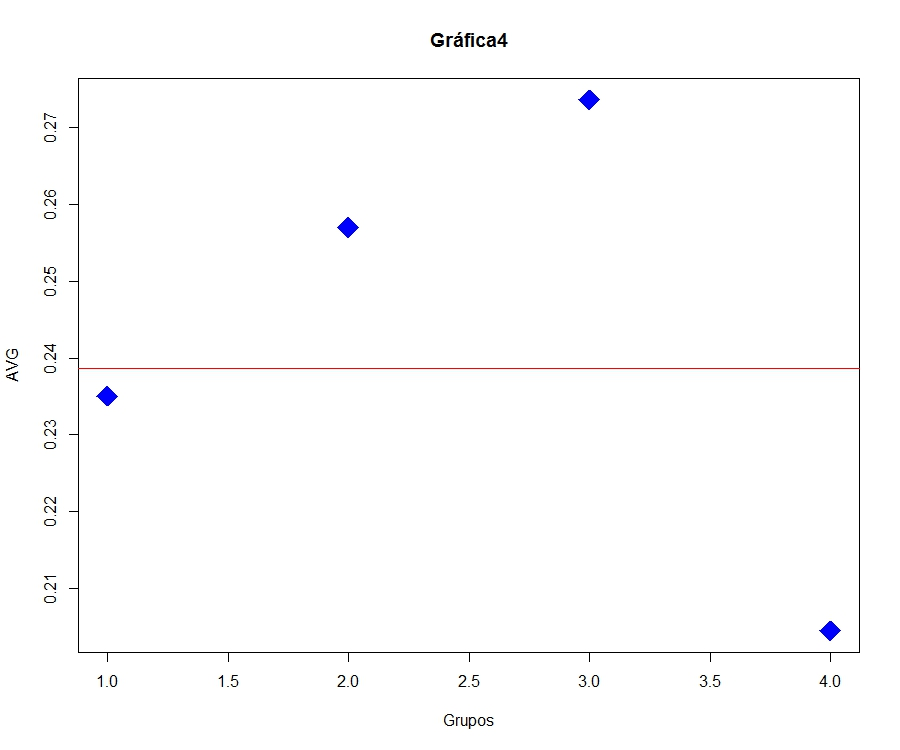
\includegraphics[scale=0.4]{Grafica4.jpeg} \vspace{1.5cm}
    	
    	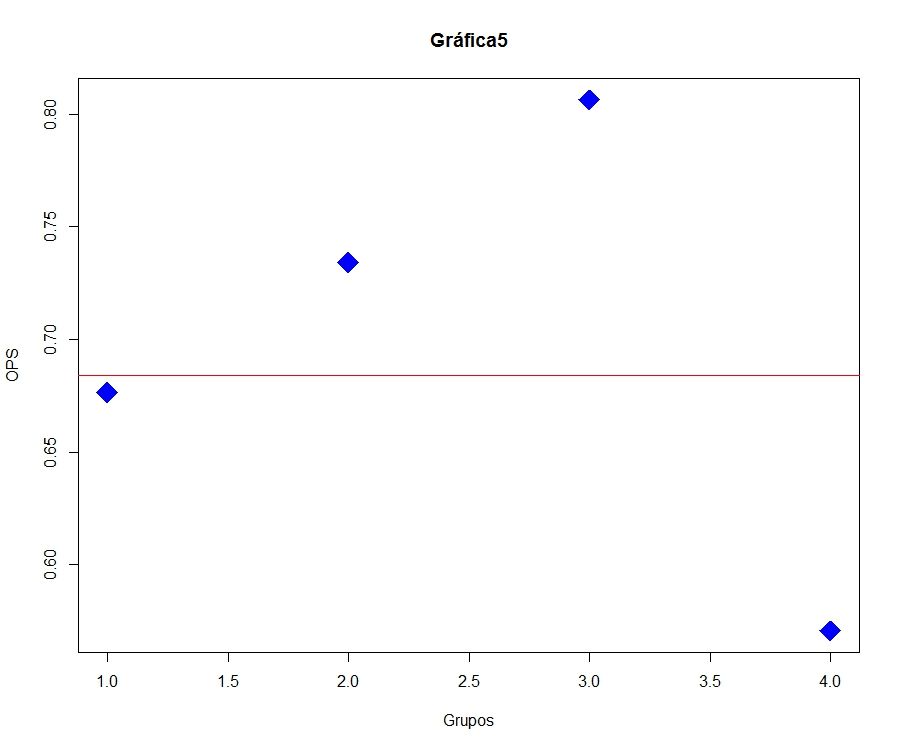
\includegraphics[scale=0.4]{Grafica5.jpeg} 
    \end{center} \newpage
    
     Ahora bien, los métodos estadísticos para llevar a cabo la investigación fueron los siguientes: \\ 
     
     Análisis de correlación el cual permite observar la relación que existe entre las variables. A su vez, la moda que es el valor que tiene mayor frecuencia absoluta en el conjunto de datos, en esta ocasión como se mencionó anteriormente fue empleada para sustituir los valores faltantes en la variable edad. \\
     
     Por otra parte, la media aritmética que es el valor promedio de las muestras y fue la principal medida que se utilizó, gracias a esta se logró clasificar a los grupos y atribuirle la etiqueta de (Bajo, Regular, Alto, Muy Alto). 
     Por último, la varianza fue considerada ya que se aplicó un análisis de los principales componentes el cual permite reducir la dimensión de las observaciones perdiendo la menor cantidad de información posible. \\ 
     \begin{center}
     	\textbf{\large  Análisis de los resultados }
     \end{center} 
    
     En la temporada regular del 2016 de la MLB  se efectuaron un total de 162 juegos. Mediante el presente trabajo de investigación se obtuvieron los siguientes resultados: \\ 
     
     
     El promedio de participación de los bateadores fue de 83 juegos, es decir, el 51\% de toda la temporada regular. Observando los 4 grupos por separado existe una gran diferencia de los jugadores que pertenecen a cada uno de estos, la cual se puede percibir de la siguiente forma:\\ 
     
     \noindent $\bullet$ El grupo 1 participó en el 46\% de los juegos.\\ 
     $\bullet$ El grupo 2 participo en el 71\% de los juegos.\\
     $\bullet$ El grupo 3 participo en el 93\% de los juegos.\\
     $\bullet$ El grupo 4 participo en el 21\% de los juegos. \\ 
     
     Esto indica que hay dos grupos que están por encima del promedio y los otros dos están por debajo. \\ 
     
     
     Otra característica que se observó fue en la variable “carreras”, en donde el máximo de carreras anotadas por un jugador en la temporada fue de 123, y el promedio general del grupo completo fue de 36 carreras, ahora bien, el promedio por grupo se refleja de la siguiente manera: el grupo 1 anotó 24 carreras, el grupo 2 anotó 49 carreras, el grupo 3 anotó 82 carreras y por último el grupo 4 anotó 5 carreras. \\
     
     En la variable home run (HR) se observó que la cantidad máxima de HR dentro de la temporada alcanzada por un jugador fue de 47 y el promedio general de HR por jugador es de 9. \\
     
     Luego examinando los grupos se obtuvo que el promedio de HR del grupo 1 fue de 5 HR, el grupo 2 de 12 HR, el grupo 3 de  23 HR y grupo 4 de 1 HR. 
     Hasta ahora se puede apreciar que el grupo 4 está muy por debajo del promedio y el grupo 3 muy por encima del promedio, con ayuda de esto y las gráficas anteriores se logró etiquetar a los jugadores según su rendimiento de la siguiente forma: \\ 
     
     \noindent $\bullet$ Grupo 1 Regular con una cantidad de 136 jugadores.\\ 
     $\bullet$ Grupo 2 Alto con una cantidad de 117 jugadores.\\
     $\bullet$ Grupo 3 Muy Alto con una cantidad de 121 jugadores.\\
     $\bullet$ Grupo 4 Bajo con una cantidad con una cantidad de 173 jugadores.\\ 
     
     
     Esto denota que el 56\% de los bateadores están por debajo del promedio en las principales características.\\
     
     Luego de finalizado el proceso de la investigación surgió una nueva inquietud, la cual arrojó la siguiente interrogante: ¿Qué equipo al terminar la temporada regular tenía mejor grupo de bateadores? \\ 
     
     Para ello se presenta la siguiente imagen que contiene la tabla:
  
  \begin{center}
  		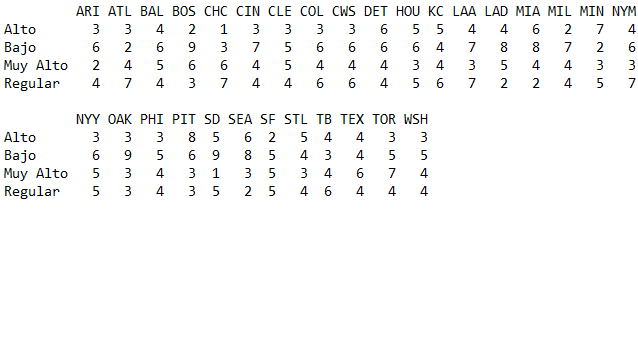
\includegraphics[scale=0.65]{equi.png}
  \end{center}
     
     De acuerdo con esta tabla, el equipo de Texas tenía el mejor grupo de bateadores al terminar la temporada regular 2016, sin embargo, el campeón fue el equipo de Chicago Cubs, lo que demuestra que un equipo para ser ganador no sólo requiere excelencia en el bateo sino también en la defensiva.
     
   
  
\end{document}
